\documentclass[1p]{elsarticle_modified}
%\bibliographystyle{elsarticle-num}

%\usepackage[colorlinks]{hyperref}
%\usepackage{abbrmath_seonhwa} %\Abb, \Ascr, \Acal ,\Abf, \Afrak
\usepackage{amsfonts}
\usepackage{amssymb}
\usepackage{amsmath}
\usepackage{amsthm}
\usepackage{scalefnt}
\usepackage{amsbsy}
\usepackage{kotex}
\usepackage{caption}
\usepackage{subfig}
\usepackage{color}
\usepackage{graphicx}
\usepackage{xcolor} %% white, black, red, green, blue, cyan, magenta, yellow
\usepackage{float}
\usepackage{setspace}
\usepackage{hyperref}

\usepackage{tikz}
\usetikzlibrary{arrows}

\usepackage{multirow}
\usepackage{array} % fixed length table
\usepackage{hhline}

%%%%%%%%%%%%%%%%%%%%%
\makeatletter
\renewcommand*\env@matrix[1][\arraystretch]{%
	\edef\arraystretch{#1}%
	\hskip -\arraycolsep
	\let\@ifnextchar\new@ifnextchar
	\array{*\c@MaxMatrixCols c}}
\makeatother %https://tex.stackexchange.com/questions/14071/how-can-i-increase-the-line-spacing-in-a-matrix
%%%%%%%%%%%%%%%

\usepackage[normalem]{ulem}

\newcommand{\msout}[1]{\ifmmode\text{\sout{\ensuremath{#1}}}\else\sout{#1}\fi}
%SOURCE: \msout is \stkout macro in https://tex.stackexchange.com/questions/20609/strikeout-in-math-mode

\newcommand{\cancel}[1]{
	\ifmmode
	{\color{red}\msout{#1}}
	\else
	{\color{red}\sout{#1}}
	\fi
}

\newcommand{\add}[1]{
	{\color{blue}\uwave{#1}}
}

\newcommand{\replace}[2]{
	\ifmmode
	{\color{red}\msout{#1}}{\color{blue}\uwave{#2}}
	\else
	{\color{red}\sout{#1}}{\color{blue}\uwave{#2}}
	\fi
}

\newcommand{\Sol}{\mathcal{S}} %segment
\newcommand{\D}{D} %diagram
\newcommand{\A}{\mathcal{A}} %arc


%%%%%%%%%%%%%%%%%%%%%%%%%%%%%5 test

\def\sl{\operatorname{\textup{SL}}(2,\Cbb)}
\def\psl{\operatorname{\textup{PSL}}(2,\Cbb)}
\def\quan{\mkern 1mu \triangleright \mkern 1mu}

\theoremstyle{definition}
\newtheorem{thm}{Theorem}[section]
\newtheorem{prop}[thm]{Proposition}
\newtheorem{lem}[thm]{Lemma}
\newtheorem{ques}[thm]{Question}
\newtheorem{cor}[thm]{Corollary}
\newtheorem{defn}[thm]{Definition}
\newtheorem{exam}[thm]{Example}
\newtheorem{rmk}[thm]{Remark}
\newtheorem{alg}[thm]{Algorithm}

\newcommand{\I}{\sqrt{-1}}
\begin{document}

%\begin{frontmatter}
%
%\title{Boundary parabolic representations of knots up to 8 crossings}
%
%%% Group authors per affiliation:
%\author{Yunhi Cho} 
%\address{Department of Mathematics, University of Seoul, Seoul, Korea}
%\ead{yhcho@uos.ac.kr}
%
%
%\author{Seonhwa Kim} %\fnref{s_kim}}
%\address{Center for Geometry and Physics, Institute for Basic Science, Pohang, 37673, Korea}
%\ead{ryeona17@ibs.re.kr}
%
%\author{Hyuk Kim}
%\address{Department of Mathematical Sciences, Seoul National University, Seoul 08826, Korea}
%\ead{hyukkim@snu.ac.kr}
%
%\author{Seokbeom Yoon}
%\address{Department of Mathematical Sciences, Seoul National University, Seoul, 08826,  Korea}
%\ead{sbyoon15@snu.ac.kr}
%
%\begin{abstract}
%We find all boundary parabolic representation of knots up to 8 crossings.
%
%\end{abstract}
%\begin{keyword}
%    \MSC[2010] 57M25 
%\end{keyword}
%
%\end{frontmatter}

%\linenumbers
%\tableofcontents
%
\newcommand\colored[1]{\textcolor{white}{\rule[-0.35ex]{0.8em}{1.4ex}}\kern-0.8em\color{red} #1}%
%\newcommand\colored[1]{\textcolor{white}{ #1}\kern-2.17ex	\textcolor{white}{ #1}\kern-1.81ex	\textcolor{white}{ #1}\kern-2.15ex\color{red}#1	}

{\Large $\underline{11a_{362}~(K11a_{362})}$}

\setlength{\tabcolsep}{10pt}
\renewcommand{\arraystretch}{1.6}
\vspace{1cm}\begin{tabular}{m{100pt}>{\centering\arraybackslash}m{274pt}}
\multirow{5}{120pt}{
	\centering
	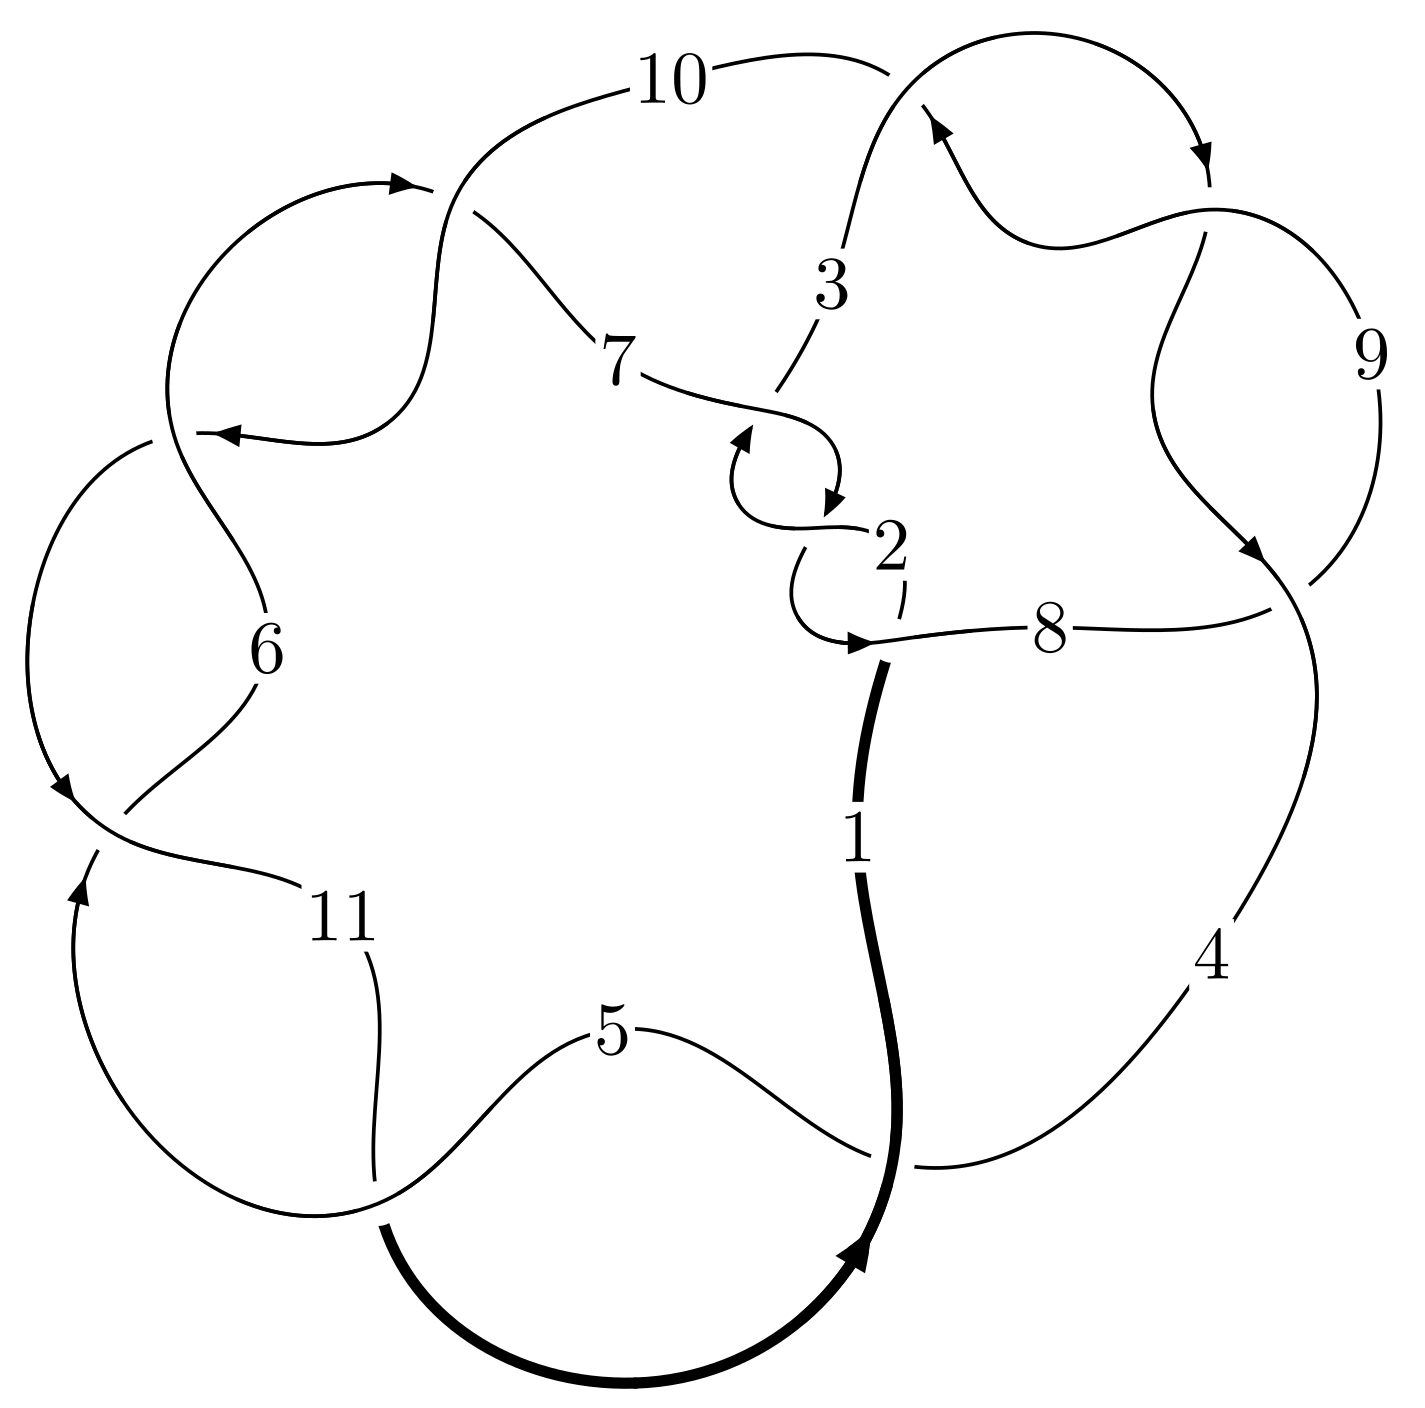
\includegraphics[width=112pt]{../../../GIT/diagram.site/Diagrams/png/611_11a_362.png}\\
\ \ \ A knot diagram\footnotemark}&
\allowdisplaybreaks
\textbf{Linearized knot diagam} \\
\cline{2-2}
 &
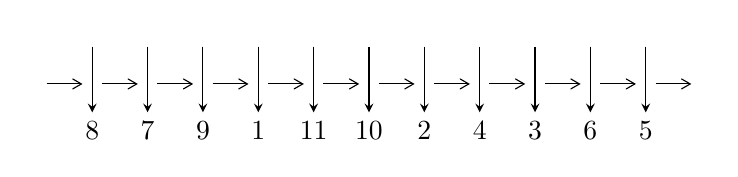
\begin{tikzpicture}[x=20pt, y=17pt]
	% nodes
	\node (C0) at (0, 0) {};
	\node (C1) at (1, 0) {};
	\node (C1U) at (1, +1) {};
	\node (C1D) at (1, -1) {8};

	\node (C2) at (2, 0) {};
	\node (C2U) at (2, +1) {};
	\node (C2D) at (2, -1) {7};

	\node (C3) at (3, 0) {};
	\node (C3U) at (3, +1) {};
	\node (C3D) at (3, -1) {9};

	\node (C4) at (4, 0) {};
	\node (C4U) at (4, +1) {};
	\node (C4D) at (4, -1) {1};

	\node (C5) at (5, 0) {};
	\node (C5U) at (5, +1) {};
	\node (C5D) at (5, -1) {11};

	\node (C6) at (6, 0) {};
	\node (C6U) at (6, +1) {};
	\node (C6D) at (6, -1) {10};

	\node (C7) at (7, 0) {};
	\node (C7U) at (7, +1) {};
	\node (C7D) at (7, -1) {2};

	\node (C8) at (8, 0) {};
	\node (C8U) at (8, +1) {};
	\node (C8D) at (8, -1) {4};

	\node (C9) at (9, 0) {};
	\node (C9U) at (9, +1) {};
	\node (C9D) at (9, -1) {3};

	\node (C10) at (10, 0) {};
	\node (C10U) at (10, +1) {};
	\node (C10D) at (10, -1) {6};

	\node (C11) at (11, 0) {};
	\node (C11U) at (11, +1) {};
	\node (C11D) at (11, -1) {5};
	\node (C12) at (12, 0) {};

	% arrows
	\draw[->,>={angle 60}]
	(C0) edge (C1) (C1) edge (C2) (C2) edge (C3) (C3) edge (C4) (C4) edge (C5) (C5) edge (C6) (C6) edge (C7) (C7) edge (C8) (C8) edge (C9) (C9) edge (C10) (C10) edge (C11) (C11) edge (C12) ;	\draw[->,>=stealth]
	(C1U) edge (C1D) (C2U) edge (C2D) (C3U) edge (C3D) (C4U) edge (C4D) (C5U) edge (C5D) (C6U) edge (C6D) (C7U) edge (C7D) (C8U) edge (C8D) (C9U) edge (C9D) (C10U) edge (C10D) (C11U) edge (C11D) ;
	\end{tikzpicture} \\
\hhline{~~} \\& 
\textbf{Solving Sequence} \\ \cline{2-2} 
 &
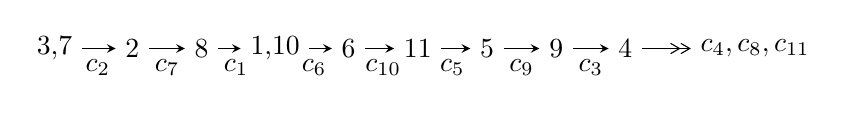
\begin{tikzpicture}[x=25pt, y=7pt]
	% node
	\node (A0) at (-1/8, 0) {3,7};
	\node (A1) at (1, 0) {2};
	\node (A2) at (2, 0) {8};
	\node (A3) at (49/16, 0) {1,10};
	\node (A4) at (33/8, 0) {6};
	\node (A5) at (41/8, 0) {11};
	\node (A6) at (49/8, 0) {5};
	\node (A7) at (57/8, 0) {9};
	\node (A8) at (65/8, 0) {4};
	\node (C1) at (1/2, -1) {$c_{2}$};
	\node (C2) at (3/2, -1) {$c_{7}$};
	\node (C3) at (5/2, -1) {$c_{1}$};
	\node (C4) at (29/8, -1) {$c_{6}$};
	\node (C5) at (37/8, -1) {$c_{10}$};
	\node (C6) at (45/8, -1) {$c_{5}$};
	\node (C7) at (53/8, -1) {$c_{9}$};
	\node (C8) at (61/8, -1) {$c_{3}$};
	\node (A9) at (10, 0) {$c_{4},c_{8},c_{11}$};

	% edge
	\draw[->,>=stealth]	
	(A0) edge (A1) (A1) edge (A2) (A2) edge (A3) (A3) edge (A4) (A4) edge (A5) (A5) edge (A6) (A6) edge (A7) (A7) edge (A8) ;
	\draw[->>,>={angle 60}]	
	(A8) edge (A9);
\end{tikzpicture} \\ 

\end{tabular} \\

\footnotetext{
The image of knot diagram is generated by the software ``\textbf{Draw programme}" developed by Andrew Bartholomew(\url{http://www.layer8.co.uk/maths/draw/index.htm\#Running-draw}), where we modified some parts for our purpose(\url{https://github.com/CATsTAILs/LinksPainter}).
}\phantom \\ \newline 
\centering \textbf{Ideals for irreducible components\footnotemark of $X_{\text{par}}$} 
 
\begin{align*}
I^u_{1}&=\langle 
b- u,\;u^{10}- u^9+7 u^8-8 u^7+17 u^6-20 u^5+14 u^4-12 u^3+4 a+9 u+1,\\
\phantom{I^u_{1}}&\phantom{= \langle  }u^{11}+8 u^9- u^8+23 u^7-5 u^6+26 u^5-6 u^4+8 u^3+u^2+2 u-1\rangle \\
I^u_{2}&=\langle 
-5 u^{11}-82 u^{10}+\cdots+547 b-41,\;572 u^{11}+957 u^{10}+\cdots+2735 a+3487,\\
\phantom{I^u_{2}}&\phantom{= \langle  }u^{12}+u^{11}+6 u^{10}+6 u^9+13 u^8+11 u^7+15 u^6+7 u^5+17 u^4+5 u^3+16 u^2+6 u+5\rangle \\
I^u_{3}&=\langle 
b+u,\;a^2- a-1,\;u^2+1\rangle \\
\\
\end{align*}
\raggedright * 3 irreducible components of $\dim_{\mathbb{C}}=0$, with total 27 representations.\\
\footnotetext{All coefficients of polynomials are rational numbers. But the coefficients are sometimes approximated in decimal forms when there is not enough margin.}
\newpage
\renewcommand{\arraystretch}{1}
\centering \section*{I. $I^u_{1}= \langle b- u,\;u^{10}- u^9+\cdots+4 a+1,\;u^{11}+8 u^9+\cdots+2 u-1 \rangle$}
\flushleft \textbf{(i) Arc colorings}\\
\begin{tabular}{m{7pt} m{180pt} m{7pt} m{180pt} }
\flushright $a_{3}=$&$\begin{pmatrix}1\\0\end{pmatrix}$ \\
\flushright $a_{7}=$&$\begin{pmatrix}0\\u\end{pmatrix}$ \\
\flushright $a_{2}=$&$\begin{pmatrix}1\\- u^2\end{pmatrix}$ \\
\flushright $a_{8}=$&$\begin{pmatrix}- u\\u^3+u\end{pmatrix}$ \\
\flushright $a_{1}=$&$\begin{pmatrix}u^2+1\\- u^4-2 u^2\end{pmatrix}$ \\
\flushright $a_{10}=$&$\begin{pmatrix}-\frac{1}{4} u^{10}+\frac{1}{4} u^9+\cdots-\frac{9}{4} u-\frac{1}{4}\\u\end{pmatrix}$ \\
\flushright $a_{6}=$&$\begin{pmatrix}-\frac{1}{2} u^{10}-4 u^8+\cdots+2 u-\frac{1}{2}\\\frac{1}{4} u^{10}-\frac{1}{4} u^9+\cdots+\frac{1}{4} u+\frac{1}{4}\end{pmatrix}$ \\
\flushright $a_{11}=$&$\begin{pmatrix}-\frac{1}{2} u^{10}-\frac{1}{2} u^9+\cdots-\frac{5}{2} u^2- u\\\frac{1}{4} u^{10}+\frac{1}{4} u^9+\cdots-\frac{1}{4} u+\frac{1}{4}\end{pmatrix}$ \\
\flushright $a_{5}=$&$\begin{pmatrix}\frac{1}{4} u^{10}+\frac{1}{4} u^9+\cdots+\frac{1}{4} u+\frac{3}{4}\\\frac{1}{4} u^{10}+\frac{1}{4} u^9+\cdots+\frac{1}{4} u-\frac{1}{4}\end{pmatrix}$ \\
\flushright $a_{9}=$&$\begin{pmatrix}-\frac{1}{4} u^{10}+\frac{1}{4} u^9+\cdots-\frac{5}{4} u-\frac{1}{4}\\u\end{pmatrix}$ \\
\flushright $a_{4}=$&$\begin{pmatrix}\frac{1}{4} u^{10}+\frac{1}{4} u^9+\cdots+\frac{1}{4} u+\frac{3}{4}\\u^2\end{pmatrix}$\\ \flushright $a_{4}=$&$\begin{pmatrix}\frac{1}{4} u^{10}+\frac{1}{4} u^9+\cdots+\frac{1}{4} u+\frac{3}{4}\\u^2\end{pmatrix}$\\&\end{tabular}
\flushleft \textbf{(ii) Obstruction class $= -1$}\\~\\
\flushleft \textbf{(iii) Cusp Shapes $= -3 u^{10}-2 u^9-24 u^8-12 u^7-66 u^6-25 u^5-65 u^4-23 u^3-11 u^2-14 u-13$}\\~\\
\newpage\renewcommand{\arraystretch}{1}
\flushleft \textbf{(iv) u-Polynomials at the component}\newline \\
\begin{tabular}{m{50pt}|m{274pt}}
Crossings & \hspace{64pt}u-Polynomials at each crossing \\
\hline $$\begin{aligned}c_{1},c_{2},c_{3}\\c_{7},c_{8},c_{9}\end{aligned}$$&$\begin{aligned}
&u^{11}+8 u^9+u^8+23 u^7+5 u^6+26 u^5+6 u^4+8 u^3- u^2+2 u+1
\end{aligned}$\\
\hline $$\begin{aligned}c_{4},c_{5},c_{6}\\c_{10},c_{11}\end{aligned}$$&$\begin{aligned}
&u^{11}+3 u^{10}+\cdots+13 u+2
\end{aligned}$\\
\hline
\end{tabular}\\~\\
\newpage\renewcommand{\arraystretch}{1}
\flushleft \textbf{(v) Riley Polynomials at the component}\newline \\
\begin{tabular}{m{50pt}|m{274pt}}
Crossings & \hspace{64pt}Riley Polynomials at each crossing \\
\hline $$\begin{aligned}c_{1},c_{2},c_{3}\\c_{7},c_{8},c_{9}\end{aligned}$$&$\begin{aligned}
&y^{11}+16 y^{10}+\cdots+6 y-1
\end{aligned}$\\
\hline $$\begin{aligned}c_{4},c_{5},c_{6}\\c_{10},c_{11}\end{aligned}$$&$\begin{aligned}
&y^{11}+15 y^{10}+\cdots+37 y-4
\end{aligned}$\\
\hline
\end{tabular}\\~\\
\newpage\flushleft \textbf{(vi) Complex Volumes and Cusp Shapes}
$$\begin{array}{c|c|c}  
\text{Solutions to }I^u_{1}& \I (\text{vol} + \sqrt{-1}CS) & \text{Cusp shape}\\
 \hline 
\begin{aligned}
u &= \phantom{-}0.412939 + 0.618853 I \\
a &= -1.86851 - 1.24582 I \\
b &= \phantom{-}0.412939 + 0.618853 I\end{aligned}
 & \phantom{-}10.82280 - 1.46957 I & -5.57474 + 4.71346 I \\ \hline\begin{aligned}
u &= \phantom{-}0.412939 - 0.618853 I \\
a &= -1.86851 + 1.24582 I \\
b &= \phantom{-}0.412939 - 0.618853 I\end{aligned}
 & \phantom{-}10.82280 + 1.46957 I & -5.57474 - 4.71346 I \\ \hline\begin{aligned}
u &= -0.360154 + 0.393035 I \\
a &= \phantom{-}1.25715 - 0.93867 I \\
b &= -0.360154 + 0.393035 I\end{aligned}
 & \phantom{-}1.95559 + 1.25455 I & -6.26218 - 5.85654 I \\ \hline\begin{aligned}
u &= -0.360154 - 0.393035 I \\
a &= \phantom{-}1.25715 + 0.93867 I \\
b &= -0.360154 - 0.393035 I\end{aligned}
 & \phantom{-}1.95559 - 1.25455 I & -6.26218 + 5.85654 I \\ \hline\begin{aligned}
u &= -0.07033 + 1.59466 I \\
a &= \phantom{-}0.276929 + 0.448902 I \\
b &= -0.07033 + 1.59466 I\end{aligned}
 & \phantom{-}10.55850 + 2.37127 I & -3.60289 - 2.68530 I \\ \hline\begin{aligned}
u &= -0.07033 - 1.59466 I \\
a &= \phantom{-}0.276929 - 0.448902 I \\
b &= -0.07033 - 1.59466 I\end{aligned}
 & \phantom{-}10.55850 - 2.37127 I & -3.60289 + 2.68530 I \\ \hline\begin{aligned}
u &= \phantom{-}0.22374 + 1.62996 I \\
a &= -0.756490 + 0.157129 I \\
b &= \phantom{-}0.22374 + 1.62996 I\end{aligned}
 & \phantom{-}15.5882 - 6.3668 I & -0.98879 + 3.90232 I \\ \hline\begin{aligned}
u &= \phantom{-}0.22374 - 1.62996 I \\
a &= -0.756490 - 0.157129 I \\
b &= \phantom{-}0.22374 - 1.62996 I\end{aligned}
 & \phantom{-}15.5882 + 6.3668 I & -0.98879 - 3.90232 I \\ \hline\begin{aligned}
u &= \phantom{-}0.314433\phantom{ +0.000000I} \\
a &= -0.886718\phantom{ +0.000000I} \\
b &= \phantom{-}0.314433\phantom{ +0.000000I}\end{aligned}
 & -0.496230\phantom{ +0.000000I} & -19.9870\phantom{ +0.000000I} \\ \hline\begin{aligned}
u &= -0.36341 + 1.67319 I \\
a &= \phantom{-}1.034280 - 0.155633 I \\
b &= -0.36341 + 1.67319 I\end{aligned}
 & -13.1804 + 8.7652 I & -0.57808 - 3.37097 I\\
 \hline 
 \end{array}$$\newpage$$\begin{array}{c|c|c}  
\text{Solutions to }I^u_{1}& \I (\text{vol} + \sqrt{-1}CS) & \text{Cusp shape}\\
 \hline 
\begin{aligned}
u &= -0.36341 - 1.67319 I \\
a &= \phantom{-}1.034280 + 0.155633 I \\
b &= -0.36341 - 1.67319 I\end{aligned}
 & -13.1804 - 8.7652 I & -0.57808 + 3.37097 I\\
 \hline 
 \end{array}$$\newpage\newpage\renewcommand{\arraystretch}{1}
\centering \section*{II. $I^u_{2}= \langle -5 u^{11}-82 u^{10}+\cdots+547 b-41,\;572 u^{11}+957 u^{10}+\cdots+2735 a+3487,\;u^{12}+u^{11}+\cdots+6 u+5 \rangle$}
\flushleft \textbf{(i) Arc colorings}\\
\begin{tabular}{m{7pt} m{180pt} m{7pt} m{180pt} }
\flushright $a_{3}=$&$\begin{pmatrix}1\\0\end{pmatrix}$ \\
\flushright $a_{7}=$&$\begin{pmatrix}0\\u\end{pmatrix}$ \\
\flushright $a_{2}=$&$\begin{pmatrix}1\\- u^2\end{pmatrix}$ \\
\flushright $a_{8}=$&$\begin{pmatrix}- u\\u^3+u\end{pmatrix}$ \\
\flushright $a_{1}=$&$\begin{pmatrix}u^2+1\\- u^4-2 u^2\end{pmatrix}$ \\
\flushright $a_{10}=$&$\begin{pmatrix}-0.209141 u^{11}-0.349909 u^{10}+\cdots-1.48702 u-1.27495\\0.00914077 u^{11}+0.149909 u^{10}+\cdots-1.71298 u+0.0749543\end{pmatrix}$ \\
\flushright $a_{6}=$&$\begin{pmatrix}0.0138940 u^{11}-0.0921389 u^{10}+\cdots+0.116271 u-0.646069\\-0.223035 u^{11}-0.257770 u^{10}+\cdots-0.603291 u-0.628885\end{pmatrix}$ \\
\flushright $a_{11}=$&$\begin{pmatrix}0.0277879 u^{11}-0.184278 u^{10}+\cdots-0.767459 u-1.29214\\0.0182815 u^{11}+0.299817 u^{10}+\cdots-0.425960 u+0.149909\end{pmatrix}$ \\
\flushright $a_{5}=$&$\begin{pmatrix}0.0197441 u^{11}-0.236197 u^{10}+\cdots+0.0599634 u-0.918099\\-0.234004 u^{11}-0.237660 u^{10}+\cdots-0.747715 u-1.11883\end{pmatrix}$ \\
\flushright $a_{9}=$&$\begin{pmatrix}-\frac{1}{5} u^{11}-\frac{1}{5} u^{10}+\cdots-\frac{16}{5} u-\frac{6}{5}\\0.00914077 u^{11}+0.149909 u^{10}+\cdots-1.71298 u+0.0749543\end{pmatrix}$ \\
\flushright $a_{4}=$&$\begin{pmatrix}-0.0149909 u^{11}-0.00585009 u^{10}+\cdots+0.769287 u-0.802925\\-0.140768 u^{11}+0.0914077 u^{10}+\cdots-0.0201097 u-0.954296\end{pmatrix}$\\ \flushright $a_{4}=$&$\begin{pmatrix}-0.0149909 u^{11}-0.00585009 u^{10}+\cdots+0.769287 u-0.802925\\-0.140768 u^{11}+0.0914077 u^{10}+\cdots-0.0201097 u-0.954296\end{pmatrix}$\\&\end{tabular}
\flushleft \textbf{(ii) Obstruction class $= -1$}\\~\\
\flushleft \textbf{(iii) Cusp Shapes $= -\frac{828}{547} u^{11}+\frac{424}{547} u^{10}-\frac{3252}{547} u^9+\frac{964}{547} u^8-\frac{2920}{547} u^7+\frac{624}{547} u^6-\frac{3248}{547} u^5+\frac{4136}{547} u^4-\frac{9020}{547} u^3+\frac{7924}{547} u^2-\frac{3244}{547} u-\frac{882}{547}$}\\~\\
\newpage\renewcommand{\arraystretch}{1}
\flushleft \textbf{(iv) u-Polynomials at the component}\newline \\
\begin{tabular}{m{50pt}|m{274pt}}
Crossings & \hspace{64pt}u-Polynomials at each crossing \\
\hline $$\begin{aligned}c_{1},c_{2},c_{3}\\c_{7},c_{8},c_{9}\end{aligned}$$&$\begin{aligned}
&u^{12}- u^{11}+\cdots-6 u+5
\end{aligned}$\\
\hline $$\begin{aligned}c_{4},c_{5},c_{6}\\c_{10},c_{11}\end{aligned}$$&$\begin{aligned}
&(u^6- u^5+5 u^4-4 u^3+6 u^2-3 u+1)^2
\end{aligned}$\\
\hline
\end{tabular}\\~\\
\newpage\renewcommand{\arraystretch}{1}
\flushleft \textbf{(v) Riley Polynomials at the component}\newline \\
\begin{tabular}{m{50pt}|m{274pt}}
Crossings & \hspace{64pt}Riley Polynomials at each crossing \\
\hline $$\begin{aligned}c_{1},c_{2},c_{3}\\c_{7},c_{8},c_{9}\end{aligned}$$&$\begin{aligned}
&y^{12}+11 y^{11}+\cdots+124 y+25
\end{aligned}$\\
\hline $$\begin{aligned}c_{4},c_{5},c_{6}\\c_{10},c_{11}\end{aligned}$$&$\begin{aligned}
&(y^6+9 y^5+29 y^4+40 y^3+22 y^2+3 y+1)^2
\end{aligned}$\\
\hline
\end{tabular}\\~\\
\newpage\flushleft \textbf{(vi) Complex Volumes and Cusp Shapes}
$$\begin{array}{c|c|c}  
\text{Solutions to }I^u_{2}& \I (\text{vol} + \sqrt{-1}CS) & \text{Cusp shape}\\
 \hline 
\begin{aligned}
u &= \phantom{-}0.778448 + 0.629355 I \\
a &= \phantom{-}0.839269 + 0.810995 I \\
b &= -0.06243 - 1.43905 I\end{aligned}
 & \phantom{-}7.93269 - 2.65597 I & -2.41885 + 3.39809 I \\ \hline\begin{aligned}
u &= \phantom{-}0.778448 - 0.629355 I \\
a &= \phantom{-}0.839269 - 0.810995 I \\
b &= -0.06243 + 1.43905 I\end{aligned}
 & \phantom{-}7.93269 + 2.65597 I & -2.41885 - 3.39809 I \\ \hline\begin{aligned}
u &= \phantom{-}0.010658 + 1.201250 I \\
a &= \phantom{-}0.301274 - 0.265056 I \\
b &= -0.293888 - 0.567347 I\end{aligned}
 & \phantom{-}3.03178 - 1.10871 I & -7.53615 + 6.18117 I \\ \hline\begin{aligned}
u &= \phantom{-}0.010658 - 1.201250 I \\
a &= \phantom{-}0.301274 + 0.265056 I \\
b &= -0.293888 + 0.567347 I\end{aligned}
 & \phantom{-}3.03178 + 1.10871 I & -7.53615 - 6.18117 I \\ \hline\begin{aligned}
u &= -1.047750 + 0.669346 I \\
a &= -0.79276 + 1.18795 I \\
b &= \phantom{-}0.11496 - 1.62096 I\end{aligned}
 & \phantom{-}18.6443 + 3.4272 I & -2.04500 - 2.25224 I \\ \hline\begin{aligned}
u &= -1.047750 - 0.669346 I \\
a &= -0.79276 - 1.18795 I \\
b &= \phantom{-}0.11496 + 1.62096 I\end{aligned}
 & \phantom{-}18.6443 - 3.4272 I & -2.04500 + 2.25224 I \\ \hline\begin{aligned}
u &= -0.293888 + 0.567347 I \\
a &= -0.730525 - 0.188448 I \\
b &= \phantom{-}0.010658 - 1.201250 I\end{aligned}
 & \phantom{-}3.03178 + 1.10871 I & -7.53615 - 6.18117 I \\ \hline\begin{aligned}
u &= -0.293888 - 0.567347 I \\
a &= -0.730525 + 0.188448 I \\
b &= \phantom{-}0.010658 + 1.201250 I\end{aligned}
 & \phantom{-}3.03178 - 1.10871 I & -7.53615 + 6.18117 I \\ \hline\begin{aligned}
u &= -0.06243 + 1.43905 I \\
a &= -0.808537 - 0.064242 I \\
b &= \phantom{-}0.778448 - 0.629355 I\end{aligned}
 & \phantom{-}7.93269 + 2.65597 I & -2.41885 - 3.39809 I \\ \hline\begin{aligned}
u &= -0.06243 - 1.43905 I \\
a &= -0.808537 + 0.064242 I \\
b &= \phantom{-}0.778448 + 0.629355 I\end{aligned}
 & \phantom{-}7.93269 - 2.65597 I & -2.41885 + 3.39809 I\\
 \hline 
 \end{array}$$\newpage$$\begin{array}{c|c|c}  
\text{Solutions to }I^u_{2}& \I (\text{vol} + \sqrt{-1}CS) & \text{Cusp shape}\\
 \hline 
\begin{aligned}
u &= \phantom{-}0.11496 + 1.62096 I \\
a &= \phantom{-}1.091280 + 0.055514 I \\
b &= -1.047750 - 0.669346 I\end{aligned}
 & \phantom{-}18.6443 - 3.4272 I & -2.04500 + 2.25224 I \\ \hline\begin{aligned}
u &= \phantom{-}0.11496 - 1.62096 I \\
a &= \phantom{-}1.091280 - 0.055514 I \\
b &= -1.047750 + 0.669346 I\end{aligned}
 & \phantom{-}18.6443 + 3.4272 I & -2.04500 - 2.25224 I\\
 \hline 
 \end{array}$$\newpage\newpage\renewcommand{\arraystretch}{1}
\centering \section*{III. $I^u_{3}= \langle b+u,\;a^2- a-1,\;u^2+1 \rangle$}
\flushleft \textbf{(i) Arc colorings}\\
\begin{tabular}{m{7pt} m{180pt} m{7pt} m{180pt} }
\flushright $a_{3}=$&$\begin{pmatrix}1\\0\end{pmatrix}$ \\
\flushright $a_{7}=$&$\begin{pmatrix}0\\u\end{pmatrix}$ \\
\flushright $a_{2}=$&$\begin{pmatrix}1\\1\end{pmatrix}$ \\
\flushright $a_{8}=$&$\begin{pmatrix}- u\\0\end{pmatrix}$ \\
\flushright $a_{1}=$&$\begin{pmatrix}0\\1\end{pmatrix}$ \\
\flushright $a_{10}=$&$\begin{pmatrix}a\\- u\end{pmatrix}$ \\
\flushright $a_{6}=$&$\begin{pmatrix}a u+u\\a+u\end{pmatrix}$ \\
\flushright $a_{11}=$&$\begin{pmatrix}- a-1\\a u- a\end{pmatrix}$ \\
\flushright $a_{5}=$&$\begin{pmatrix}- a u\\- a u-1\end{pmatrix}$ \\
\flushright $a_{9}=$&$\begin{pmatrix}a- u\\- u\end{pmatrix}$ \\
\flushright $a_{4}=$&$\begin{pmatrix}- a u\\-1\end{pmatrix}$\\ \flushright $a_{4}=$&$\begin{pmatrix}- a u\\-1\end{pmatrix}$\\&\end{tabular}
\flushleft \textbf{(ii) Obstruction class $= 1$}\\~\\
\flushleft \textbf{(iii) Cusp Shapes $= 0$}\\~\\
\newpage\renewcommand{\arraystretch}{1}
\flushleft \textbf{(iv) u-Polynomials at the component}\newline \\
\begin{tabular}{m{50pt}|m{274pt}}
Crossings & \hspace{64pt}u-Polynomials at each crossing \\
\hline $$\begin{aligned}c_{1},c_{2},c_{3}\\c_{7},c_{8},c_{9}\end{aligned}$$&$\begin{aligned}
&(u^2+1)^2
\end{aligned}$\\
\hline $$\begin{aligned}c_{4},c_{5},c_{6}\\c_{10},c_{11}\end{aligned}$$&$\begin{aligned}
&u^4+3 u^2+1
\end{aligned}$\\
\hline
\end{tabular}\\~\\
\newpage\renewcommand{\arraystretch}{1}
\flushleft \textbf{(v) Riley Polynomials at the component}\newline \\
\begin{tabular}{m{50pt}|m{274pt}}
Crossings & \hspace{64pt}Riley Polynomials at each crossing \\
\hline $$\begin{aligned}c_{1},c_{2},c_{3}\\c_{7},c_{8},c_{9}\end{aligned}$$&$\begin{aligned}
&(y+1)^4
\end{aligned}$\\
\hline $$\begin{aligned}c_{4},c_{5},c_{6}\\c_{10},c_{11}\end{aligned}$$&$\begin{aligned}
&(y^2+3 y+1)^2
\end{aligned}$\\
\hline
\end{tabular}\\~\\
\newpage\flushleft \textbf{(vi) Complex Volumes and Cusp Shapes}
$$\begin{array}{c|c|c}  
\text{Solutions to }I^u_{3}& \I (\text{vol} + \sqrt{-1}CS) & \text{Cusp shape}\\
 \hline 
\begin{aligned}
u &= \phantom{-0.000000 -}1.000000 I \\
a &= -0.618034\phantom{ +0.000000I} \\
b &= \phantom{-0.000000 } -1.000000 I\end{aligned}
 & \phantom{-}4.27683\phantom{ +0.000000I} & \phantom{-0.000000 } 0 \\ \hline\begin{aligned}
u &= \phantom{-0.000000 -}1.000000 I \\
a &= \phantom{-}1.61803\phantom{ +0.000000I} \\
b &= \phantom{-0.000000 } -1.000000 I\end{aligned}
 & \phantom{-}12.1725\phantom{ +0.000000I} & \phantom{-0.000000 } 0 \\ \hline\begin{aligned}
u &= \phantom{-0.000000 } -1.000000 I \\
a &= -0.618034\phantom{ +0.000000I} \\
b &= \phantom{-0.000000 -}1.000000 I\end{aligned}
 & \phantom{-}4.27683\phantom{ +0.000000I} & \phantom{-0.000000 } 0 \\ \hline\begin{aligned}
u &= \phantom{-0.000000 } -1.000000 I \\
a &= \phantom{-}1.61803\phantom{ +0.000000I} \\
b &= \phantom{-0.000000 -}1.000000 I\end{aligned}
 & \phantom{-}12.1725\phantom{ +0.000000I} & \phantom{-0.000000 } 0\\
 \hline 
 \end{array}$$\newpage
\newpage\renewcommand{\arraystretch}{1}
\centering \section*{ IV. u-Polynomials}
\begin{tabular}{m{50pt}|m{274pt}}
Crossings & \hspace{64pt}u-Polynomials at each crossing \\
\hline $$\begin{aligned}c_{1},c_{2},c_{3}\\c_{7},c_{8},c_{9}\end{aligned}$$&$\begin{aligned}
&((u^2+1)^2)(u^{11}+8 u^9+\cdots+2 u+1)\\
&\cdot(u^{12}- u^{11}+\cdots-6 u+5)
\end{aligned}$\\
\hline $$\begin{aligned}c_{4},c_{5},c_{6}\\c_{10},c_{11}\end{aligned}$$&$\begin{aligned}
&(u^4+3 u^2+1)(u^6- u^5+5 u^4-4 u^3+6 u^2-3 u+1)^2\\
&\cdot(u^{11}+3 u^{10}+\cdots+13 u+2)
\end{aligned}$\\
\hline
\end{tabular}\newpage\renewcommand{\arraystretch}{1}
\centering \section*{ V. Riley Polynomials}
\begin{tabular}{m{50pt}|m{274pt}}
Crossings & \hspace{64pt}Riley Polynomials at each crossing \\
\hline $$\begin{aligned}c_{1},c_{2},c_{3}\\c_{7},c_{8},c_{9}\end{aligned}$$&$\begin{aligned}
&((y+1)^4)(y^{11}+16 y^{10}+\cdots+6 y-1)(y^{12}+11 y^{11}+\cdots+124 y+25)
\end{aligned}$\\
\hline $$\begin{aligned}c_{4},c_{5},c_{6}\\c_{10},c_{11}\end{aligned}$$&$\begin{aligned}
&(y^2+3 y+1)^2(y^6+9 y^5+29 y^4+40 y^3+22 y^2+3 y+1)^2\\
&\cdot(y^{11}+15 y^{10}+\cdots+37 y-4)
\end{aligned}$\\
\hline
\end{tabular}
\vskip 2pc
\end{document}